\clearpage
\begin{center}
	\section*{\large{CHAPTER III \\ \vspace{-0.3cm} RESEARCH METHODOLOGY}}
\end{center}
\addcontentsline{toc}{section}{\textbf{CHAPTER III: RESEARCH METHODOLOGY }}
\renewcommand{\thepage}{\arabic{page}}
\setstretch{1.3}
This section discusses the theoretical and conceptual framework of the study. Sustainable rural livelihood framework proposed by  \citet{dfid1999sustainable} and Household Vulnerability assessment framework approach is used to examine the Household vulnerability. The following sections describes the sample design, conceptual frame work , sources of data and techniques for data analysis. \\

\subsection*{3.1  Philosophical Issues}
\addcontentsline{toc}{subsection}{3.1  Philosophical Issues}
\renewcommand{\thepage}{\arabic{page}}
\setstretch{1.3}
This study adopts a research paradigm influenced by radical structuralism, which assumes that household vulnerability and coping capacity is objectively determined by factors such as Social Asset, Human Asset, Natural Asset, Financial Asset, and Physical Asset. The ontological position of this study is objectivism, as it aims to produce objective and value-free knowledge about reality as a part of economics research. The epistemological position is positivism, as it relies on empirical methods and data to develop and test theories of Household Vulnerability. The axiological position is value-free, as the researcher endeavors to not be influenced by or influence the subject or results of the study. The philosophical tradition that guides this study is the Neo-classical framework.\par

\subsection*{3.2 Research Design}
\addcontentsline{toc}{subsection}{3.2 Research Design}
\renewcommand{\thepage}{\arabic{page}}
\setstretch{1.3}
The research is based on descriptive and analytical research design. The objective of the research is to assess the household-level vulnerability and coping capacity. The variables related to Social Asset, Human Asset, Natural Asset, Financial Asset, and Physical Asset were included at the time of Household-level vulnerability index. The variables are: Household head age, Hosuehold head educational attainment, Highest educational attainment of the household, Number of male adults, Number of childrens, Number of female adults, Number of Elders, Debt of the household, Land owned by the household, Saving of the household, Jewellery of the household. The index were then employed to assess the household's vulnerability and variability in relation to other households in the same village of the districts of concern.   


\subsection*{3.3 Conceptual Framework}
\addcontentsline{toc}{subsection}{3.3 Conceptual Framework}
\renewcommand{\thepage}{\arabic{page}}
\setstretch{1.3}
The conceptual framework for the first research objective is shown in figure 3.1 on the following page. In the figure, we present the sources of household vulnerability. Total of five components comprise of this conceptual framework. They are: Human Capital; Physical Capital; Livelihood; Social Capital; Financial Capital. Using the variables, we construct the Household vulnerability index. 

Similarly, figure 3.2 represents the conceptual framework for the second objective of the thesis. The figure shows that Household vulnerability as an dependent variable. Meanwhile, Environmental dependence is considered the main explanatory variable. We used both year control and time-invariant controls such as districts and VDCs. 

\subsubsection*{3.3.1. Household Vulnerability Index}
\addcontentsline{toc}{subsection}{\ \ \ \ \ 3.3.1 Household Vulnerability Index}
\renewcommand{\thepage}{\arabic{page}}
\setstretch{1.5} 
A household confronted with a difficult situation is at risk of potential future declines in welfare. Vulnerability, which is the probability of encountering future loss of welfare, typically takes into account the severity of anticipated losses. The level of vulnerability is influenced by both the nature of the risk and the household's capacity to address risk using the capitals they possess. Households face numerous uncertain events. A household is said to be vulnerable, if it doesn't have adequate resources or capitals, particularly when exposed to risky situations where the household needs to use the resources at their disposal. Those resources are capital or assets of the households. Having these resources not only helps the houeholds deal with uncertain events but also improve their livelihoods and lifestyles. 

To identify the different levels of vulnerability amongst the households in rural households, we construct the Household Vulnerability Index. Taking into the capitals that households possess, we construct an aggregated index which helps to identify the vulnerable households within the community. The capitals we use to construct the index are: Human; Physical; Social; Financial; and livelihood strategies.  
\\
\\
\\
\\
\\
\begin{figure}[H]
	\centering
	\includegraphics[scale=0.8]{Graphs and figures/Conceptual framework for Household Vulnerability Index1.png}
	\captionsetup{labelformat=empty}
	\caption{Figure 3.1: Schematic of objective one} 
	\label{fig:conceptualfw1}
\end{figure}
\subsubsection*{3.3.2. Household Vulnerability and Environmental Dependence}
\addcontentsline{toc}{subsection}{\ \ \ \ \ 3.3.2 Household Vulnerability and Environmental Dependence}
\renewcommand{\thepage}{\arabic{page}}
\setstretch{1.5} 
After we construct the index and identify the most and least vulnerable, we attempt to understand the effects of the factors that weren't included in the index construction. These variables represent the liability to a household. Environmental income is a semi-capital/semi-liability characteristics variable. Environmental income is the revenue that a household generates from forest as well as non-forest sources. The sources are natural forest, managed forest, plantations, agroforests, silvipasture, other agriculture land, other areas. The products are firewood, charcoal, poles and other building material, fodder, fish, fruits, vegetables, medicinal plants etc. Because the income from the environment is a predominant source of income for livelihoods of rural households, it can be a source of capital for those households who do not have adequate resources. But, on the other hand, it can also be a liability when depending solely on these sources. Particularly, in the context of climate change and environmental degradation, it can be a source of liability of households. So, we investigate the influence of Environmental dependence on the household vulnerability. 
\begin{figure}[h]
	\centering
	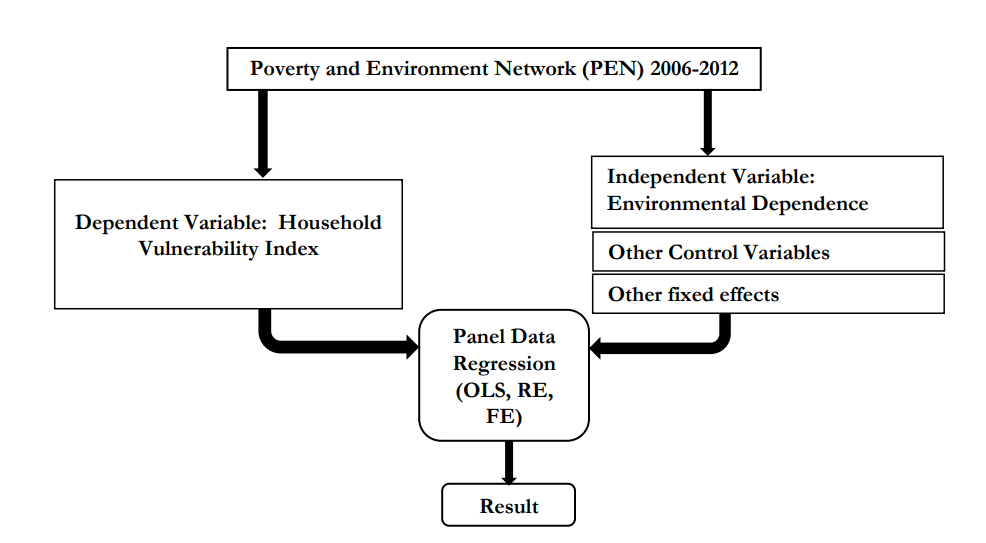
\includegraphics[scale=0.9]{Graphs and figures/Objective 2.png}
	\captionsetup{labelformat=empty}
	\caption{Figure 3.2: Schematic of objective two} 
	\label{fig:conceptualfw2}
	\setlength{\abovecaptionskip}{4pt}
\end{figure}
\\
\\
\\
\\
\\
\\
\subsection*{3.4 Sources and Nature of the Data}
\addcontentsline{toc}{subsection}{3.4 Sources and Nature of the Data}
\renewcommand{\thepage}{\arabic{page}}
\setstretch{1.5}
The sources and nature of the data are explained in this section. Further, the operationalization of the is also discussed in this section.

This study employs the A unique environmental augmented household-level livelihood panel dateset \citep{walelign2022unique} from
Nepal, Full Panel 2006-2012, produced by Tribhuvan University’s Institute of Forestry and the University of Copenhagen’s Department of Food and Resource Economics . It is a geographically representative survey spanning three main physio-graphic regions of Nepal. Data was collected in the districts of Chitwan (lowland), Kaski (mid-hills), and Mustang (mountains). Total of 507, 446 and 428 randomly sampled households were surveyed in the year 2006, 2009 and 2012 respectively. For the questionnaire see \cite{larsen2014role}. \\
The three primary physio-graphic regions of Nepal—the lowlands, mid-hills, and mountains—are covered by the study sites. The selection factors included the following: (i) Nepal's changes in elevation and vegetation; (ii) the environmental reliance of households; (iii) the attitudes of communities toward long-term research; and (iv) village accessibility and researcher safety (because of the ongoing civil conflict in Nepal at the time of site selection in 2005).\\
The data was collected through the Community Based Forest Management in the Himalaya
(ComForM) phases I - III collaborative project conducted by the Institute of Forestry (IOF) at Tribhuvan University and the Department of Food and Resource Economics (IFRO) at the University
of Copenhagen, with support from the Department of Forest Research and Survey (DFRS) at the
Ministry of Forests and Soil Conservation, Nepal. The questionnaire design was developed together with the Poverty Environment Network (PEN).\\
\begin{figure}[H]
	\centering
	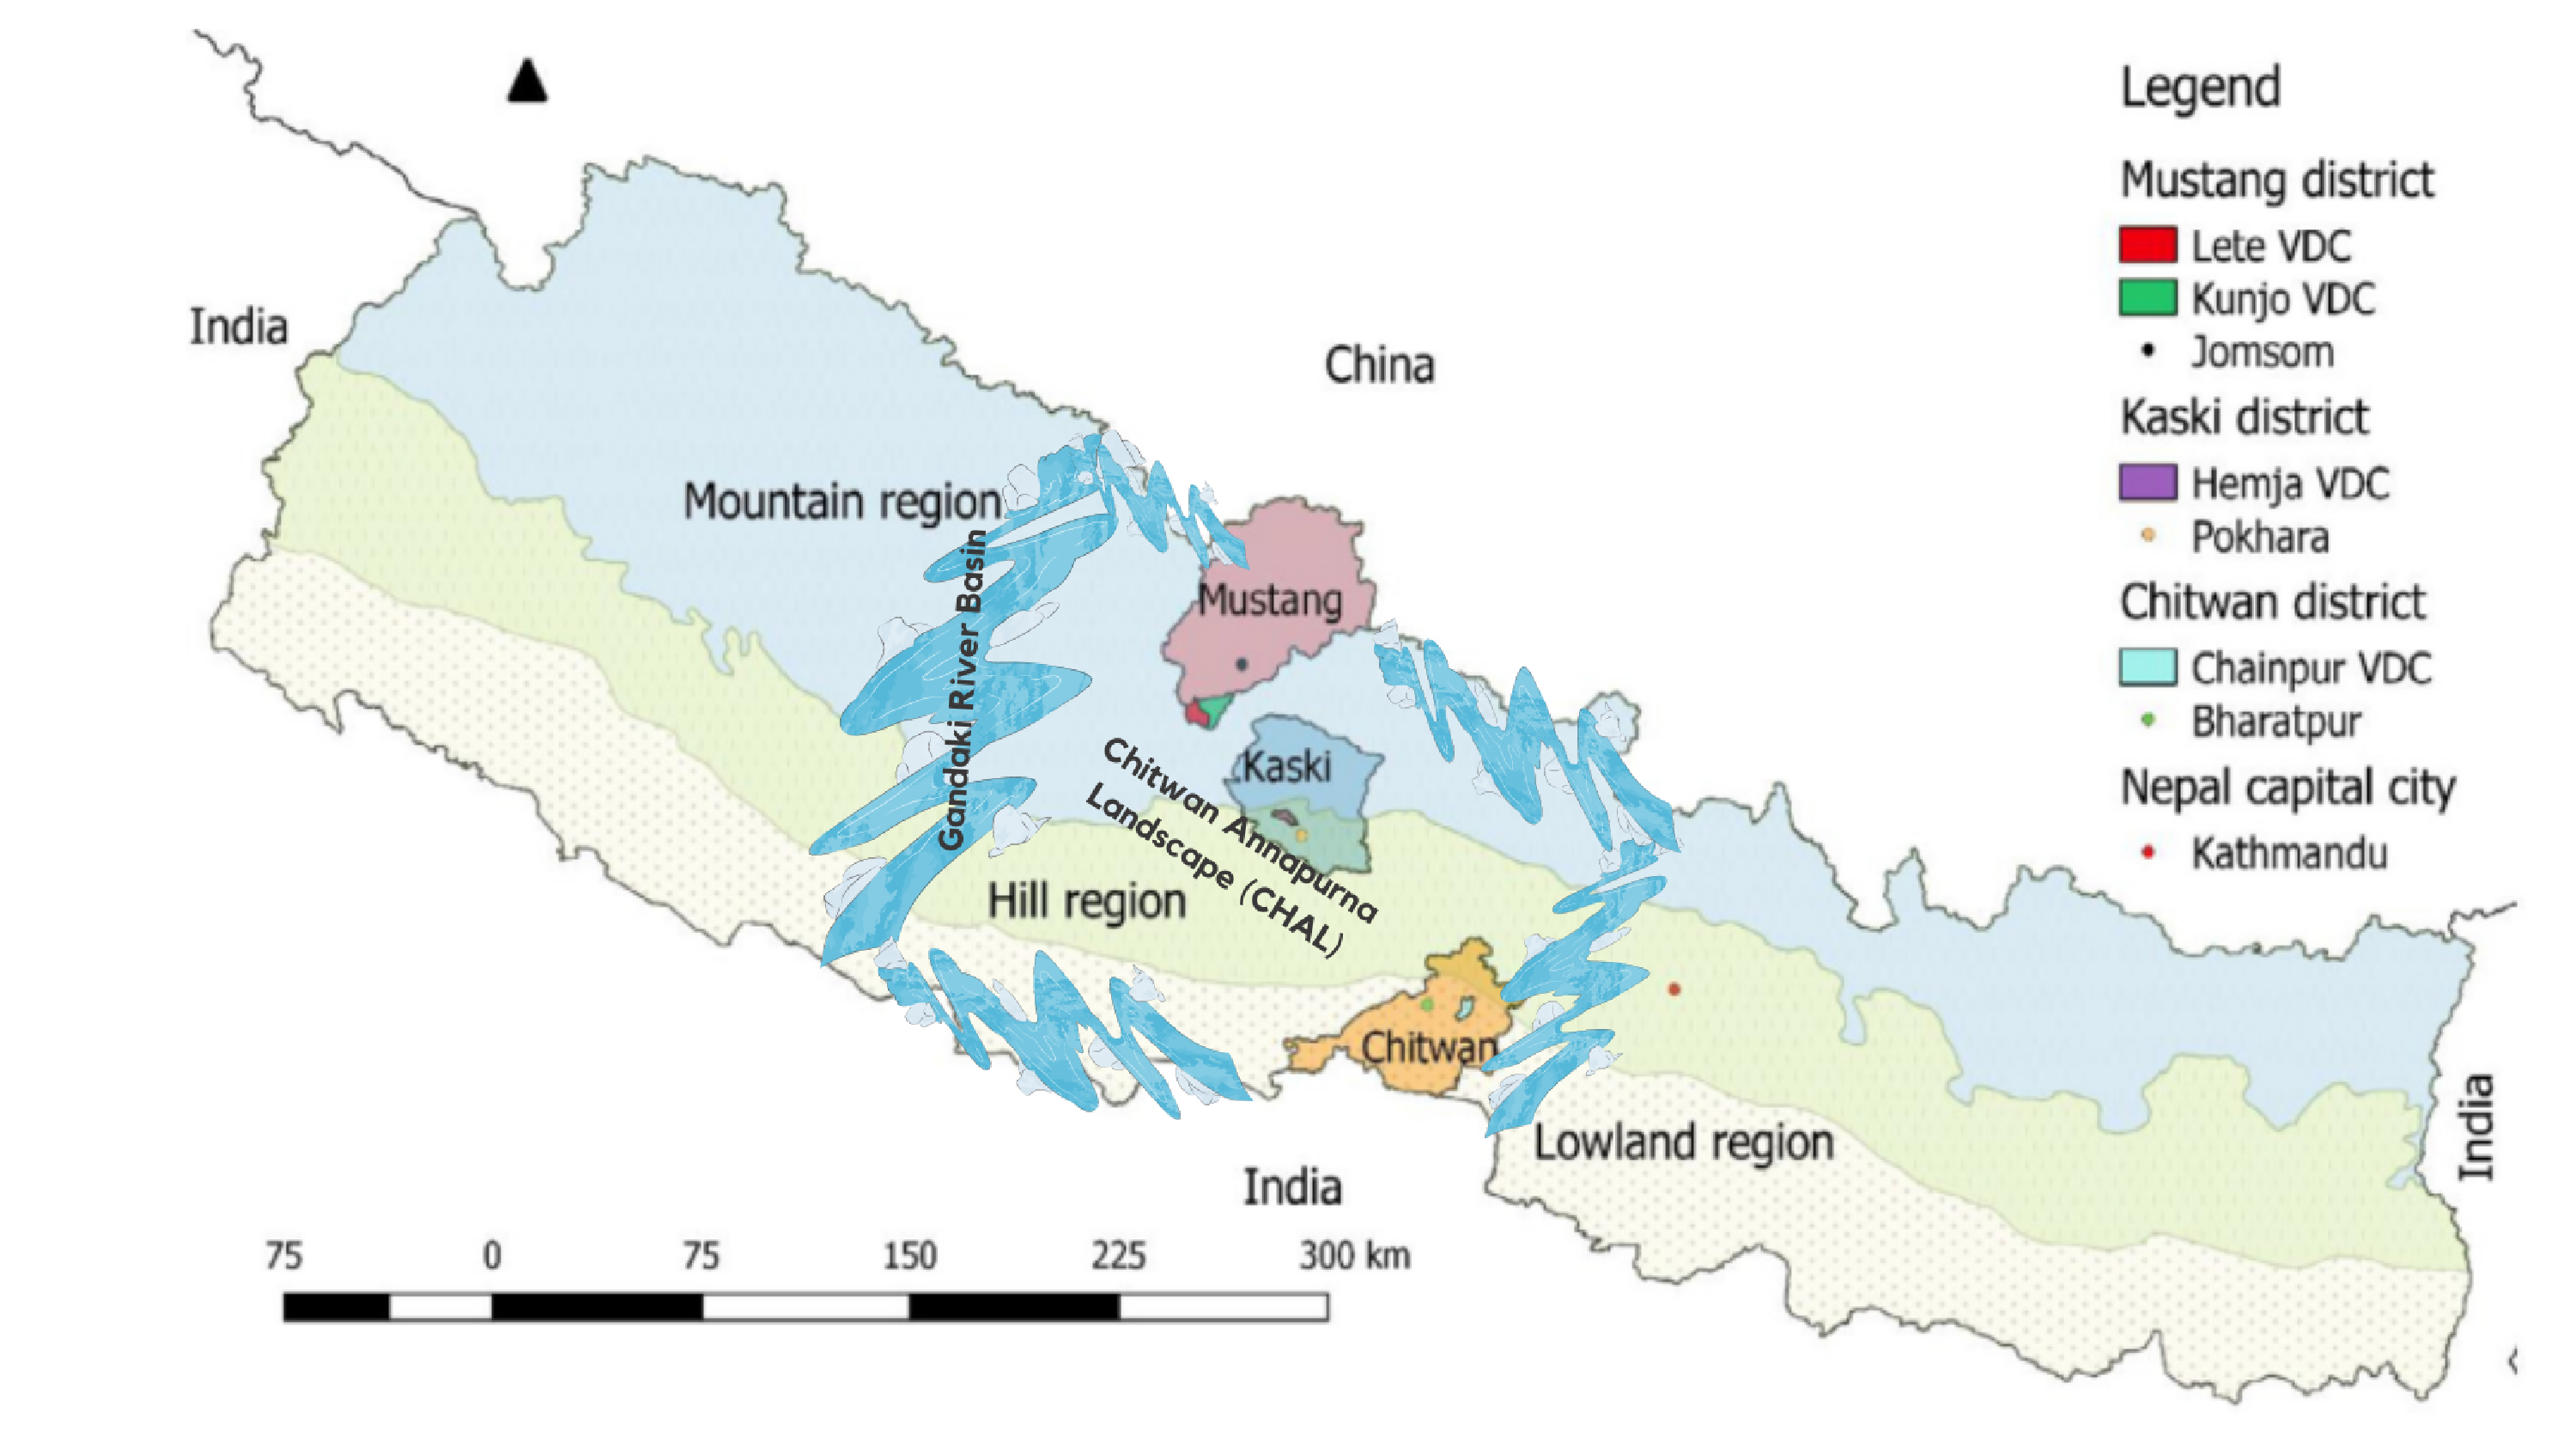
\includegraphics[scale=0.31]{Graphs and figures/Study site.png}
	\caption*{Figure 3.3: Map of the survey districts and VDCs}
	\label{fig:Surveymap}
\end{figure}

We construct the HVI as a barometer
to evaluate the level of household vulnerability at the micro
level. We constructed HVIs whose values are expressed on an interval scale
of 0-1, where the value of 0 indicates that the household is at the
minimum level of vulnerability (least vulnerable) and the value 1 indicates that the household is at the maximum vulnerability (most
vulnerable).
In order to construct the HVI, we first normalize the variables using the equations (3.5) and (3.6). The variables used are in Table 3.1. After the normalization, we grouped the variables into the group of capitals the variables belongs using equation (3.7). The we find the HVI for each household using (3.8).
\begin{singlespace}
	\centering
	\begin{table}[H]
		\captionsetup{labelformat=empty}
		\caption{Table 3.1: Definition of Variables used for HVI Construction}
		\vspace{0.05cm}
		\renewcommand{\arraystretch}{1.4}
		\resizebox{1.1\textwidth}{!}{%
			\begin{tabular}{p{3cm}p{12cm}} \hline \hline
				Variables & Construct \\ \hline
				hhh\_age & Household head age in years \\
				hhh\_edu & Education attainment of household head \\
				max\_hh\_edu & Highest educational attainment by a household member\\
				implements & Total value of implements such as: Car; Trucks; Motorbike; Plough etc. owned by the household in Rs.\\
				livestock & Total value of livestock (of all types) in Rs.\\
				land & Total area of land owned by the household in sq. m\\
				hh\_caste & Household belonging to the biggest caste in the village (=1) \\
				bank\_saving & Households savings kept in banks or other recognized financial institutions\\
				jewellery & Households' saving in the form of non-productive assets, such as Jewellery. \\
				n\_livelihoods & Count of livelihoods of the households \\ \hline \hline 
			\end{tabular} \\ 		
		}\\ 
		\small{\textit{Source: PEN Dataset}}
	\end{table} 
\end{singlespace}
HVI is then considered the outcome variable in the model (3.9) whereas Environmental dependence, as measured by ratio of Environmental Income to Total income of the households, is the the independent variables. Using the model, we investigate the effect of the Environmental dependence on the Household vulnerability.

\begin{center}
	\begin{table}[ht]
		\renewcommand{\arraystretch}{1.2} 
		\captionsetup{labelformat=empty}
		\caption{Table 3.2: Definition of Variables affecting HVI}
		\vspace{0.05cm}
		\resizebox{1\textwidth}{!}{
			\begin{tabular}{p{3cm}p{11cm}} \hline \hline
				Variables & Construct\\ \hline
				env\_dependence & Measured by the ratio of Environmental Income to Total income of the household \\
				dependency\_ratio & Measured by the ratio of dependent and working adult members of the household \\
				debt & Debt of the household in Rs. household member \\
				n\_shocks & Count of the shocks experienced by the households \\ 
				\hline \hline 
			\end{tabular} \\
		}
		\small{\textit{Source: PEN Dataset}}
	\end{table}
\end{center}
\subsection*{3.5 Techniques of Data Analysis}
\addcontentsline{toc}{subsection}{3.5 Techniques of Data Analysis}
\renewcommand{\thepage}{\arabic{page}}
\setstretch{1.5}
Household vulnerability indicators were selected after thoroughly reviewing the 
available literature.All indicators and their descriptions 
and sources are summarized in Table 3.1. The techniques of data analysis are elaborated upon in the following sections. 
\subsubsection{3.5.1. Household Vulnerability Index}
\addcontentsline{toc}{subsection}{\ \ \ \ \ 3.5.1 Household Vulnerability Index}
\renewcommand{\thepage}{\arabic{page}}
\setstretch{1.5}
To ensure the comparability of indicators that were used in the construction of the
household vulnerability index, all indicators were standardised following the
\citep{watkins2007human} procedure of standardising indicators for life expectancy index. This
ensures that all indicators were normalised to have a relative position between 0 and 1. \\
All variables with different scales are normalized with the following Min-Max standardization 
(Equations 3.5 and 3.6). Min-Max normalization helps to resize/rescale all variables analogously 
(i.e., into one scale). Here, all values are scaled between 0 and 1. Equation (3.5) applies to 
variables positively associated with vulnerability, while 
equation (3.6) applies to variables negatively associated with vulnerability. This method has been widely used in the literature related to vulnerability assessment. \cite{fang2016rural, antwi2013characterising, karunarathne2020developing, huynh2018multi, dumenu2020social} are some of the literature that have employed mini-max/maxi-min normalization technique to construct the vulnerability index.

When the variable has upward functional relationship with vulnerability, normalization was done using (3.5) and when the variable has downward functional relationship with vulnerability, normalization was done using equation (3.6):
\begin{align}
	\text{X}_{\text{ij}} &= \frac{X_{\text{i}} - X_{\text{Minj}}}{X_{\text{Maxj}} - X_{\text{Minj}}} \tag{3.5} \\[1cm] 	
	\text{X}_{\text{ij}} &= \frac{X_{\text{Maxj}} - X_{\text{i}}}{X_{\text{Maxj}} - X_{\text{Minj}}} \tag{3.6}
\end{align} 
where X is the observed value of the variable related to household i in district j, and Xmax and Xmin are 
maximum and minimum values of each variable, respectively. After normalizing all variables, 
we used equation (3.7) to calculate the final normalized index for each key component.
\begin{align}
	\text{HVI}_{\text{Cij}} &= \frac{1}{n}\sum_{i=1}^{n}\text{X}_{\text{ij}} \tag{3.7}
\end{align}
where $\text{HVI}_{\text{Cij}}$ is one of the five key components for HH. The main elements include human capital (C1), physical capital (C2), social capital (C3), livelihood (C4) and financial capital (C5). 	$\text{index}_{\text{Hvi}}$
depicts the variables of the key component indexed by C for i household in j district (while n represents the number of variables for each component). We used equation (3.8) to 
calculate the overall Hvi for the HH.
\begin{align}
	\text{HVI}_{\text{ij}} &= \sum_{i=1}^{n}\text{HVI}_{\text{Cij}} \tag{3.8}
\end{align}
where HVI is the Multi-facet Composite Household Vulnerability Index for HH x. 
C represents the numbers of key components,  indicates the weighting schemes used for the 
composite index, and n ensures the number of key components. Table 3 illustrates the weighting 
schemes used for the composite index calculated. 
\subsubsection{3.5.2. Household Vulnerability and Environmental Dependence}
\addcontentsline{toc}{subsection}{\ \ \ \ \ 3.5.2 Household Vulnerability and Environmental Dependence}
\renewcommand{\thepage}{\arabic{page}}
To examine the effect of Environmental dependence on Household vulnerability, this study employs panel estimation techniques, including pooled-OLS, fixed effects (FE), and random effects (RE) models. While simple pooled-OLS doesn't account for the time-specific or hosuehold-specific effects, the fixed effects and random effects models are designed to address such endogenity issues. Pooled-OLS is essentially a statistical regression analysis method that visually represents the relationship between data points and determines the best-fit line for a dataset. However, the fixed effects model is theoretically more suitable for cases involving unobservable individual  or household effects that may be correlated with the variables included in the model. Conversely, if individual effects are strictly uncorrelated with explanatory variables, the random effects model is a preferable choice \citep{hsiao2022analysis}.   Effect of Environmental dependence on household vulnerability is modeled using
following regression,
\vspace{-\baselineskip}
\begin{center}
	\begin{align}
		\mathit{HVI}_{i,t} &= \beta_{0} + \delta \mathit{\mathbf{ED}_{i,t}} + \mathbf{X}_{i,t} \beta + \mathbf{Z}_i \lambda + \mathbf{T}_t \delta_t + \boldsymbol{\epsilon}\tag{3.9}
	\end{align}
\end{center}
where, \textit{HVIi,t} is Household Vulnerability of $i^{th}$ household in \textit{t} year, \textit{EDi,t} is Environmental dependence, \textit{T} is year control variable, \textit{Xi,t} is the variables controlled for, which includes Dependency ratio, log of debt, count of shock experienced and \textit{Zi,t} represents control for time invariant
fixed effect such as district and VDCs and $\beta_{0}, \delta, \beta, \lambda, \delta_t$ are the parameter of the model.

\subsubsection{3.5.3. Diagnostic Tests}
\addcontentsline{toc}{subsection}{\ \ \ \ \ 3.5.3. Diagnostic Tests}
\renewcommand{\thepage}{\arabic{page}}
For each techniques of the Panel data analysis, we'll run few diagnostic tests to check for the effects to be included in the model such as Individual and Time effects. Also, we run the efficiency test for choosing between the models.

\subsubsection{3.5.3.1 Individual Effects Test}
\renewcommand{\thepage}{\arabic{page}}
We run the Pooled Ordinary Least Squares (OLS) regression model without considering individual effects. After obtaining the results from Pooled OLS regression, we conduct F-test to determine if there are significant individual effects (fixed effects) present in the model. We'll refer to the F-statistic and associated P-value to determine the presence of significant individual effects.  A low p-value suggests the presence of significant individual effects.

\subsubsection{3.5.3.2 Time Fixed Effects Test}
\renewcommand{\thepage}{\arabic{page}}
We also test for if there are time effects in the model. For this, we run the Pooled Ordinary Least Squares (OLS) regression model without considering individual effects. After obtaining the results from Pooled OLS regression, we conduct the Lagrange Multiplier Test - \cite{honda1988size}. It will allow us to determine if there are significant time effects (fixed effects) present in the model. We'll refer to the t-statistic and associated P-value to determine the presence of significant individual effects.  A low p-value suggests the presence of significant time effects.

\subsubsection{3.5.3.3 Breusch-Pagan Lagrange Multiplier (BPLM) Test}
\renewcommand{\thepage}{\arabic{page}}
This test is commonly referred to as Pool-ability test conducted for confirming if the cross-sectional unit in the panel has the same intercept or a different intercept. \cite{breusch1980lagrange} assesses the pool-ability of the data after incorporating the time and individual fixed effects. We'll analyze the test-statistic and associated p-value. A low p-value suggests that the data is not poolable, indicating the inadequacy of Pooled OLS regression. We'll go for Random effects (RE) regression if the p-value is low.

\subsubsection{3.5.3.4 Hausman Specification Test}
If the BP-LM test suggests that the data is not pool-able and suggests to go for Random Effects (RE) model, we'll run the RE regression. We'll also run the Fixed effects (FE) model to compare the result. After running both Random Effects (RE) and Fixed Effects (FE) models, conduct the Hausman Specification test \cite{hausman1978specification} to determine the efficient model. The test is to check whether the coefficients estimated by the two models are significantly different. We'll analyze the test statistic, typically a chi-square value, and assesses the associated p-value.  
